\subsection{Experiment 1 Analysis Results} \label{results-1-quan}
In this section, 
we will first present descriptive statistics 
of the raw data in our first experiment. 
Then, we will explain our feature engineering 
and data transformation process 
based on the raw data. 
Lastly, we will introduce the Bayesian Model 
we applied in our analysis 
and present the analysis results.

\subsubsection{Descriptive Statistics of the Raw Data}
% -- raw data
%     describe the dataset, total # of participants in each group before and after dataset cleaning, demographics of each group;
    
Overall, we collected 223 complete responses in the first experiment. 
We removed four poor-quality responses 
either participant responded the qualitative question facetiously 
or misunderstanding the prompt. 
Among the 219 remaining responses, 
56 completed the Likert path, 
and the rest were distributed relatively evenly 
across the remaining six subgroups with various orders of QV, 
ranging from 24 to 28 responses per subgroup. 
Aggregating responses from all six subgroups, 
the number of responses collected for QV with 36 credits (QV36), 
QV with 108 credits (QV108) and QV with 324 credits (QV324) 
were 107, 108, and 111, respectively. 
%(To-do: maybe add a hierarchical graph the represents how responses from different paths are aggregated)

We recruited the participants 
to construct a sample 
representative of the US 2019 census data 
in terms of age and education level. 
Having a representative sample is critical because of the generalizability of voting and survey tools. 
Based on Table \ref{table:demo_exp1}, 
all the groups followed the demographics in both age and education level. 
This ensured unbiased results toward any subgroup of the population, 
which is generally hard to achieve in MTurk studies without specific control \cite{difallah2018demographics}.

\begin{table}
    \centering
    \caption{
        Experiment one's sample demographics statistics aligns closely with 2019 US census across all groups and subgroup.
    }
    \Description[Experiment one's sample demographics statistics aligns closely with 2019 US census across all groups and subgroup.]{
        Experiment one's sample demographics statistics aligns closely with 2019 US census across all groups and subgroup.
    }
    \label{table:demo_exp1}
    \begin{tabular}{|c|ccccc|c|} 
    \hline
     & \begin{tabular}[c]{@{}c@{}}Likert\\Perc \end{tabular} & \begin{tabular}[c]{@{}c@{}}QV36\\Perc \end{tabular} & \begin{tabular}[c]{@{}c@{}}QV108\\Perc \end{tabular} & \begin{tabular}[c]{@{}c@{}}QV324\\Perc \end{tabular} & \begin{tabular}[c]{@{}c@{}}Total\\Perc \end{tabular} & \begin{tabular}[c]{@{}c@{}}Census\\Perc* \end{tabular} \\ 
    \hline
    No High School & 16.07\% & 14.02\% & 13.89\% & 14.41\% & 14.61\% & 10.22\% \\
    High School & 25.00\% & 27.10\% & 25.93\% & 26.13\% & 26.03\% & 27.73\% \\
    Some College  Associate & 28.57\% & 26.17\% & 34.26\% & 34.23\% & 32.88\% & 33.09\% \\
    Bachelor's Degree above & 30.36\% & 32.71\% & 34.26\% & 34.23\% & 32.88\% & 33.09\% \\ 
    \hline
    18 - 24 & 21.43\% & 15.89\% & 14.81\% & 15.32\% & 16.89\% & 13.65\% \\
    25 - 39 & 26.79\% & 29.91\% & 30.56\% & 29.73\% & 29.22\% & 30.74\% \\
    40 - 54 & 25.00\% & 29.91\% & 28.70\% & 29.73\% & 28.31\% & 28.32\% \\
    55 - 69 & 26.79\% & 24.30\% & 25.93\% & 25.23\% & 25.57\% & 27.29\% \\
    \hline
    \end{tabular}
    \vspace{-10px} %tempoary
\end{table}

% donation descriptive statistics: perc of non-zero donation, total donation amount comparison across groups, donation distribution across topics between groups
We can match each survey response, 
either a Likert or QV response,
to the set of donation decisions
made by a participant.
Since we use the donation outcome of a participant 
as a proxy of their true preferences 
across the nine societal causes, 
we could only analyze
participants who donated a non-zero amount of money.
Therefore, we further filtered the dataset 
to keep only the responses 
that had a non-zero total donation amount.
Across all the conditions, 
the average non-zero donation rate was $73.3\%$,
consistent with the results provided by \textcite{fehr2007human} in \citeyear{fehr2007human},
which suggested that about $30\%$ of the population 
would always free-ride in public goods provision 
regardless of what others do. 
The donation rate in each condition 
closely centered around the average donation rate, 
ranging from $70.37\%$ (in QV108) and $77.19\%$ (in Likert).
The number of valid responses after filtering out zero-donation participants for
Likert, QV36, QV108, and QV324 were $44$, $76$, $76$ and $84$ respectively.

Among those who donated a non-zero amount,
participants exhibited different behaviors
when deciding how much to donate in total. 
Figure \ref{fig:total_don_exp1} demonstrates
two clusters for the total donation amount. 
The first cluster centered around $\$9-12$
with the majority in the range of $\$5$ to $\$20$. 
This group of people,
making up about $60\%$ of the entire sample, 
donated part of the lottery winning amount
but still kept a significant portion for themselves.
The other clustered around $\$33$ to $\$35$, 
suggesting that this group of participants
contributed almost the full amount of the lottery prize. 
There were approximately $25\%$ of the participants who behaved this way. 
The distribution pattern across 
four surveying methods were relatively consistent, 
except that almost twice the proportion of participants 
in the Likert condition donated almost the full amount 
compared to the other QV conditions.
One possible explanation for the difference is 
the Likert group required less effort compared to that of QV, 
and participants felt less tempted 
to earn an extra reward for their time spent in the Likert condition. 
Overall, we found that the total amount of donation per participant 
was large enough to be distributed across charities
in a way that could represent the full picture of 
their true underlying preferences for nine topics.

\begin{figure}[htpb]
    \centering
    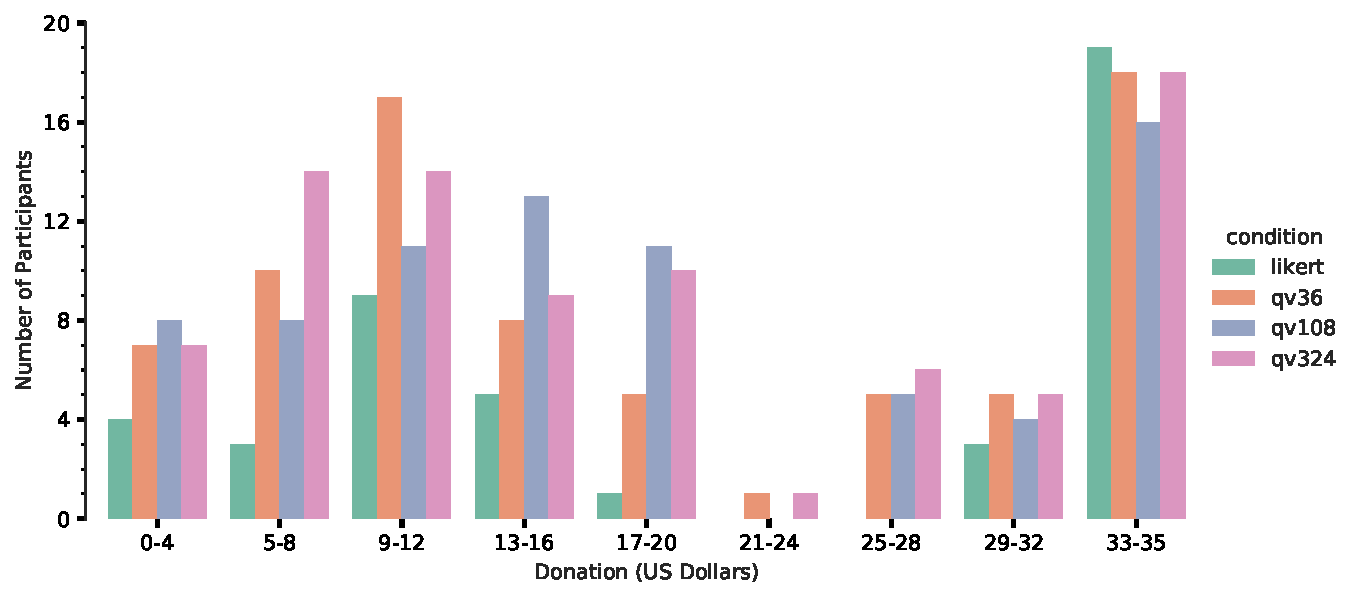
\includegraphics[width=\textwidth, keepaspectratio=true]{content/image/total_contributions_across_conditions.pdf}
    \caption{
       Distributions of the total amount donated by participants across four surveying methods.
       We see two distributions, one centered by $\$9-12$ and the other centered by $\$33$ to $\$35$.
       We also see more Likert participants donate almost most of their donation quota compared to the QV Groups.
    }
    \Description[Distributions of Total Donation Amounts across Groups for experiment 1]{ Distributions of the total amount donated by participants across four surveying methods.
    We see two distributions, one centered by $\$9-12$ and the other centered by $\$33$ to $\$35$.
    We also see more Likert participants donate almost most of their donation quota compared to the QV Groups.}
    \label{fig:total_don_exp1}
\end{figure}

Aggregated across all participants,
the amount of donations for each 
of the nine charities have a similar trend
shown in Figure \ref{fig:topic_don_exp1}. 
Environment-related, health-related, and human-related charities 
were consistently the more popular 
compared to the art-related, international-related, and faith-related charities.
However, there are some differences 
when observing the population-level preferences 
towards charities across the four surveying methods. 
For example, the pets-related charity 
received far less donation in percentage 
for the Likert Group compared with the QV groups. 
This suggests that there was a good amount of variance 
in people's opinions toward the nine topics, 
making the surveying task meaningful.

\begin{figure}[htpb]
    \centering
    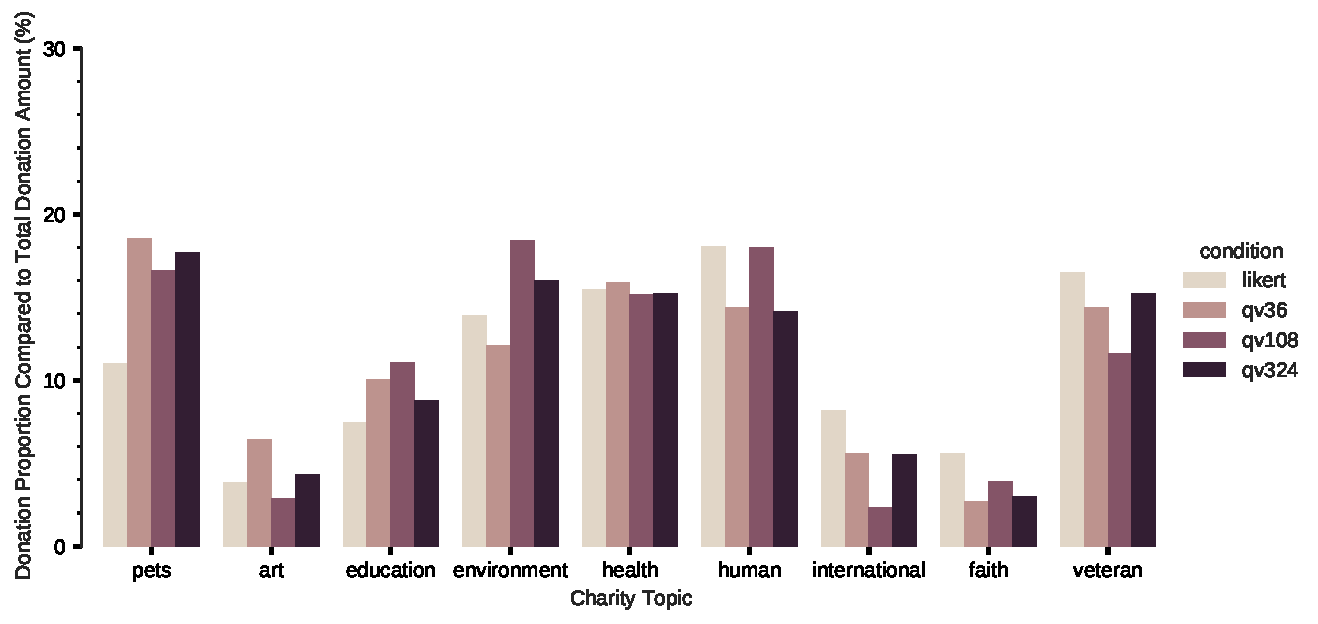
\includegraphics[width=\textwidth, keepaspectratio=true]{content/image/normalized_contributions_per_topic_across_conditions.pdf}
    \caption{
      Percentage Contribution Amount per Topic with Respect to the Total Donation Amount across Conditions.
      We see a general trend of the more and less popular charities while some differences across each
      surveying method within each group.
    }
    \Description[Percentage Contribution Amount per Topic with Respect to the Total Donation Amount across Conditions for experiment 1]{
      Percentage Contribution Amount per Topic with Respect to the Total Donation Amount across Conditions.
      We see a general trend of the more and less popular charities while some differences across each
      surveying method within each group.
    }
    \label{fig:topic_don_exp1}
\end{figure}

\begin{figure}[htpb]
    \centering
    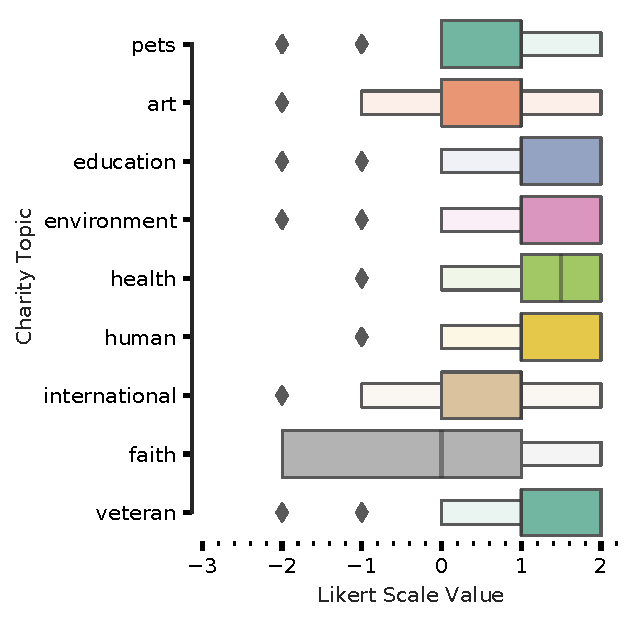
\includegraphics[width=0.4\textwidth, keepaspectratio=true]{content/image/likert_distribution_per_topic.pdf}
    \caption{
      Distribution of Likert Responses per Topic. 
      Each level from -2 to 2 corresponds to 
      ``Very unimportant'', ``Unimportant'', ``Neutral'', ``Important'', and ``Very important''.
      We see a right skewed distribution across all groups with variations in their shapes.
      This means that participants showed their relative preferences even in the Likert Group.
    }
    \Description[Distribution of Likert Responses per Topic for experiment 1]{Distribution of Likert Responses per Topic for experiment 1}
    \label{fig:likert_exp1}
\end{figure}

%     QV & Likert votes descriptive statistics: votes distribution per topic across groups, budget usage distribution across QV groups

Figure \ref{fig:likert_exp1} demonstrates 
the aggregated Likert responses
distributed across the nine societal causes. 
we can see that most topics skewed towards positive opinions, 
with a median of "Important" and "Very Important." 
Despite six out of nine topics have a median of "Important," 
the shapes of their distributions are different which
suggested participants have different levels of support. 
The sufficient amount of variations 
shown across topics indicated that 
our prompt in the experiment, 
which we reminded participants that resources are limited
and one should express their relative preferences 
worked as intended. 

Comparing across the three QV surveys, 
the response distributions are similar 
but have subtle differences. 
Consistent with prior work in QV \cite{quarfoot2017quadratic}, 
most distributions of all the topics 
are close to a Normal distribution.
There is less variation
at the median of a distribution, 
comparing results from QV36 
then those from QV108 and QV324
and resembles that from the Likert survey more.
The medians of QV108 and QV324, on the contrary, 
clearly show nuanced differences across topics. 
Besides, distributions in QV324 
have longer tails 
then those in QV108, 
suggesting that participants 
did make use of the increased credits 
to express more extreme opinions at higher costs. 
After examining
the usage of 
voice credits across the three QV conditions 
(Figure \ref{fig:qv3_exp1}), 
we found no decrease 
in the median with increased budget size (all around 98\%), 
but the tail of lower percentage usage in QV324 was longer 
then in the other two cases. 
This finding assured that 
participants made good use of 
the extra credits 
and they were comfortable 
completing QV with a large budget 
up to the order of $N^2$ ($N$ is the number of options in a survey) 
and complicated calculations with our QV interface. 
% mention the implication of longer tail in QV324 in the discussion section: 
% need to be aware of using an overly large budget and resulting in a worse tail

\begin{figure}[htpb]
    \centering
    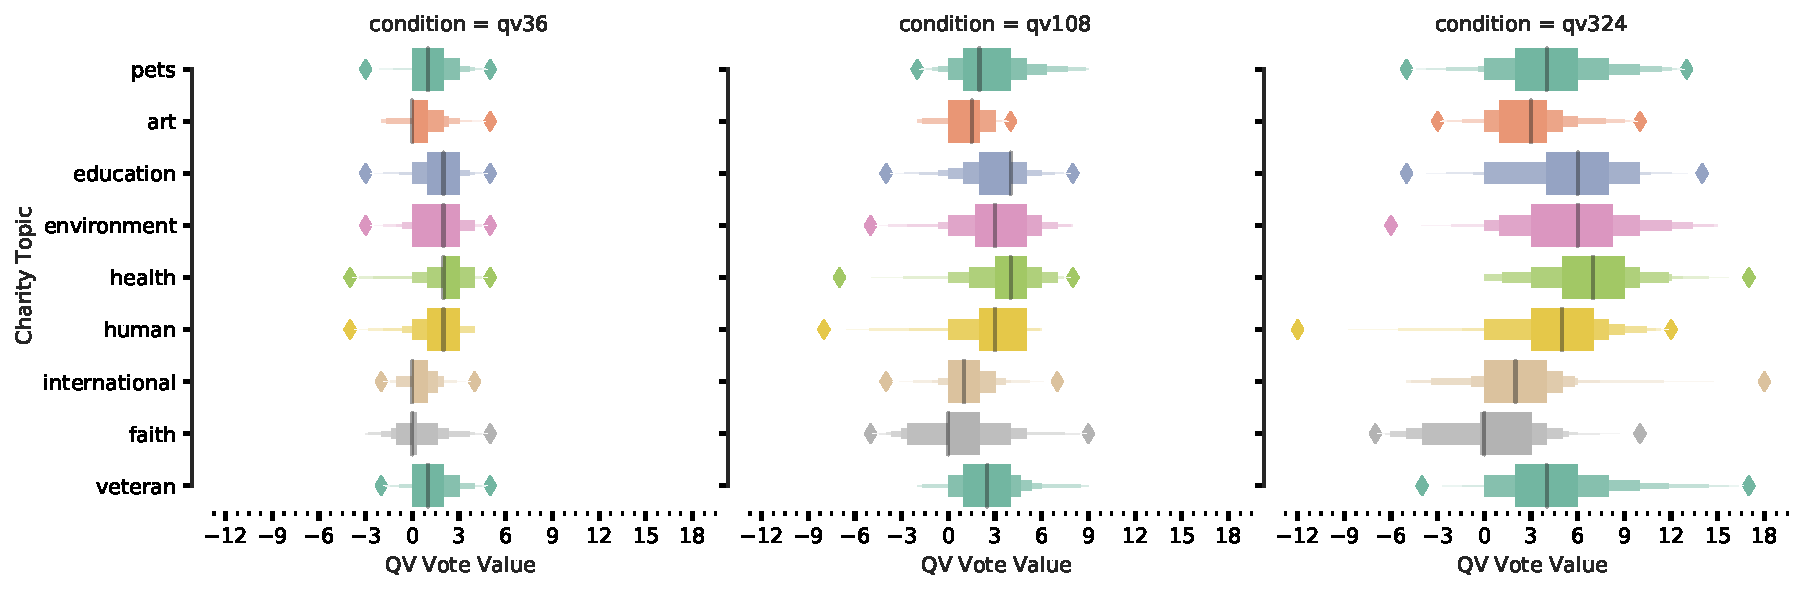
\includegraphics[width=\textwidth, keepaspectratio=true]{content/image/qv_distribution_per_topic.pdf}
    \caption{
      Distribution of QV Responses per Topic in QV36, QV108 and QV324. 
      The maximum possible number of votes on a topic was 6 votes in QV36, 10 votes in QV108, and 18 votes in QV324.
      The tails expends out as the number of total credits increases. 
      All three QV follows a normal distribution.
    }
    \Description[Distribution of QV Responses per Topic for experiment 1]{Distribution of QV Responses per Topic for experiment 1}
    \label{fig:qv3_exp1}
\end{figure}


\subsubsection{Opinions Alignment Measurement Calculation}
% -- data transformation to alignment measurement
%     describe the calculation of cosine similarity angle theta
%     mention our test of checking if other factors impact total donation amount -> absolute vs. normalized donation amount
%     show histogram and other descriptive statistics of the angle data

To answer our research question 
of how to align Likert and QV survey responses are 
with people's true opinions 
reflected by their incentive-compatible behavior, %to-do: is it accurate to use this term here?
we need to design a metric 
that can measure the degree of alignment 
between the two. 
Before discussing our choice of metric, 
we first clarify the definition of "alignment" in our analysis. 
A perfect alignment 
between a survey response 
and the same participant's donation choices
requires an individual to express their preferences
with the same relative strength as their donation amount. 
More formally, it is defined as the following:\par

\begin{quote}
    A set of survey response $\vec{v} = [v_1, v_2, ..., v_n]$, 
    and a set of donation amount $\vec{d} = [d_1, d_2, ..., d_n]$, 
    where $n$ is the number of topics or options involved in the decision, 
    are perfectly align if there exists a positive constant $k>0$ that satisfies $k\vec{v} = \vec{d}$.
\end{quote}

Our alignment focused on the relative strength across opinions for two reasons. 
First, the results from our four types of surveys 
and the donation task were not on the same scale. 
For example, the maximum possible number of votes on a topic 
in QV36 is 6 
while the maximum donation amount on a topic is \$35. 
Second, 
any two participants might donate differently
due to other factors such as income level or level of education,
even if both of them split their total donation amounts in the same way proportionally.
In other words, 
participants might donate with the \textit{same} level of preference acorss options 
but with \textit{different} levels of total amount to donate.
Hence, we decided to care only about the relative strength in opinions across topics.

The metric for measuring the degree of alignment 
thus need to be monotonic 
with respect to the amount of discrepancy 
between two preference vectors 
in terms of relative strength in preferences. 
It would be preferable if the metric is easily interpretable. 
With these two criteria in mind, 
we decided to use the angle $\theta$ in the Cosine similarity metric 
as the alignment metric. 
It is formally defined as the following: \par

\begin{quote}
    The Cosine similarity angle $\theta$ between a set of survey response $\vec{v} = [v_1, v_2, ..., v_n] \in \mathbb{R}^n$, and a set of donation amount $\vec{d} = [d_1, d_2, ..., d_n] \in \mathbb{R}^n$, where $n$ is the number of topics or options involved in the decision, is calculated via $\theta = \frac{180}{\pi} \arccos{\frac{\vec{v} \cdot \vec{d}}{\|\vec{v}\| \|\vec{d}\|}}$, and $0\deg \leq \theta \leq 180\deg$.
\end{quote}

Cosine similarity is a commonly used similarity metric 
that measures the cosine of the angle 
between two non-zero vectors \cite{singhal2001modern}. 
It only provides information about 
the relative orientation 
of the two vectors and 
does not take into account 
the magnitude of the vectors. 
Instead of resulting in a value between $0$ and $1$,
we use the the angle degree for Cosine similarity,
which represents the same information 
but provides more intuition for interpretation.
%The definition of the angle of Cosine similarity fits our need perfectly. 
It is monotonic with respect to 
how different the orientations of the two vectors are,
i.e., the relative strength in opinions, 
and does not care about the magnitude of the vectors, 
i.e., absolute vote or donation amount. 
Two sets of perfectly align opinions 
will yield a Cosine similarity angle of zero, 
while two sets of completely opposite opinions 
will result in an angle of 180 degree.

Intuitively,
to compute the Cosine similarity angle 
for each participant in each group,
we first translate each response,
urvey results from Likert, QV36, QV108, QV324, and 
their corresponding truthful preferences 
reflected in the donation task,
into a vector.
For the Likert group, 
we computed the Cosine similarity angle of a vector 
of Likert responses (between -2 and 2 for each topic) and 
a vector of the absolute donation amount of the same individual. 
In the 3 QV conditions, 
the angle is between a vector of QV votes and 
a vector of the absolute donation amount of the same participant. 
The next step is to set up a Bayesian Model 
for these four sets of Cosine similarity angle 
per condition as described in the next subsection.


\subsubsection{Bayesian Formulation}
% -- Bayesian formulation
%     why Bayesian
%     the type of analysis question
%     choice of the likelihood function
%     choice of prior distributions

Given the four sets of Cosine similarity angle 
under Likert, QV36, QV108, and QV324 conditions respectively, 
we employed a Bayesian formulation of the problem 
to compare the degree of alignment between pairs of the conditions. 
\textcite{kay2016researcher} introduced a few potential benefits 
for applying Bayesian analysis in the HCI community. 
A recent study by \textcite{xiao2019should} 
justified their use of Bayesian formulation 
with two additional reasons. 
Based on benefits proposed by past studies, 
we argued for our choice of Bayesian formulation 
with the following three reasons:

\begin{itemize}
    \item \textbf{Transparency and Fewer Assumptions} 
    In a t-test or ANOVA, 
    the data needs to follow several assumptions, 
    including Normality and Homogeneity of variance. 
    In our case, both assumptions may be violated. 
    Hence, we used Bayesian formulation 
    to relax the assumptions of normality and 
    equal variances by defining 
    a non-normal likelihood function 
    and making variances independent across groups.
    \item \textbf{Small $n$ Studies} 
    Traditional statistical tests 
    that assume normality 
    required at least a sample size of 30. 
    Even when a sample size is greater than 30, 
    a large effect size may still produce 
    an insignificant p-value 
    due to a not sufficiently large sample. 
    On the contrary, 
    a Bayesian model is valid at every value of $n$. 
    Given the relatively small sample 
    of our Likert group, 
    we chose to use a Bayesian model.
    \item \textbf{Additional Information} 
    Compared to traditional statistical analysis 
    that only produce a single p-value 
    and a single effect size value, 
    a Bayesian model is able to produce 
    the entire distribution of the effect size, 
    making additional information available 
    for clearer inference. 
    In our study, 
    effect size is in particularly important 
    because the cost of switching to a new survey tool 
    is not worthwhile 
    if the effect size is not substantial 
    even if we get a significant p-value.
\end{itemize}

In our Bayesian formulation, 
the outcome variable $\theta_{i|j}$ 
is the Cosine similarity angle 
between a survey response vector and 
a donation amount vector of each participant $i$ 
under a given experimental condition $j$: 
Likert donation alignment, QV36 donation alignment, 
QV108 donation alignment, and QV324 donation alignment. 
Our goal is to first find four best fitting distributions
that describe the four sets of $\theta_{i|j}$ respectively, 
then compare the means of each pair of distributions 
to see if they differ significantly 
and substantially via Bayesian analysis.

\begin{figure}[htpb]
    \centering
    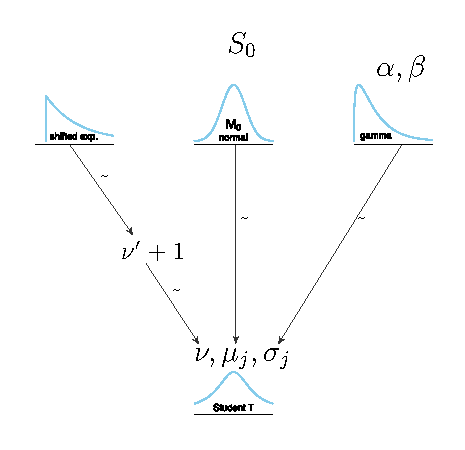
\includegraphics[width=0.6\textwidth, keepaspectratio=true]{content/image/model_1_diagram.pdf}
    \caption{
      Graphical representation of our Bayesian model \tc{Not sure how to add more details to this graph.})
    }
    \Description[Graphical representation of our Bayesian model for experiment 1]{Graphical representation of our Bayesian model for experiment 1}
    \label{fig:bayesian_model_exp1}
\end{figure}

We chose a Student-t distribution 
to describe the Cosine similarity angle data per condition, 
i.e., as the likelihood function in the Bayesian model %this sentence is unclear?
(note that this is a drawing distribution, not the t-test). 
A Student-t distribution is similar to a Normal distribution 
in the overall shape but is heavy-tailed, 
which is more forgiving about having more extreme values 
than a Normal distribution with the same variance. 
We did not want to make the strong assumption of normality 
and thus decided on a Student-t distribution. 
In Bayesian modeling, typically, the likelihood function is parametric, 
meaning that each parameter of the likelihood function is treated as a random variable 
drawn from a distribution with parameters, 
i.e., what we also called the prior of the likelihood model parameters. 
In a Student-t distribution of a given condition $j$, 
there are three parameters: 
the mean ($\mu_j$), the scale ($\sigma_j$), and the degrees of freedom ($\nu$). 
In general, we defined the priors, 
i.e., likelihood functions of the parameters, 
based on the criterion of being weakly informative 
since we did not want to impose any strong assumption on what the model should look like 
and preferred allowing all possible values for the parameters. 
The detail Bayesian model is the following (also in Fig. \ref{fig:bayesian_model_exp1}:

\begin{quote}
    $\theta_{i|j} \sim$ Student-t$(\nu, \mu_j, \sigma_j)$, \hfill likelihood function to model angle in condition $j$ (1) \\
    $\nu \sim 1 + exp(\lambda)$, \hfill degrees of freedom (2) \\
    $\mu_j \sim N(M_0, SD_0)$, \hfill modal angle in condition $j$ (3) \\
    $\sigma_j \sim \Gamma(\alpha, \beta)$, \hfill scale parameter for condition j (4)
\end{quote}

We drew the degrees of freedom $\nu$ 
from a shifted exponential distribution 
to ensure that $\nu \geq 1$. 
The mode $\mu_j$ for condition $j$ was drawn 
from a Normal distribution 
with mean $M_0$ and scale $SD_0$, 
where $M_0$ and $SD_0$ were constants that were weakly informative. 
The scale parameter $\sigma_j$ was drawn from a Gamma distribution 
with generous $\alpha$ and $\beta$ constant values 
to ensure the scale parameter was always greater than zero. (\lwt{to-do: do I need to specifiy what the constants are?})
Now that we have finished introducing our Bayesian model, 
we present the results of our analysis.

\subsubsection{Results Analysis}
    
% -- Results analysis
%     Tools: PyMC3, MCMC, NUTS
%     Describe fitted values & convergence (trace plots)
%     Describe effect size analysis for comparing Likert and QV
%     Describe effect size analysis for comparing across QVs

The Bayesian analysis was performed using PyMC3 \cite{salvatier2016probabilistic}, 
a popular Bayesian inference framework. 
One of the common computational techniques 
for Bayesian inference is Markov Chain Monte Carlo (MCMC), 
a stochastic sampling technique. 
It samples the posterior distribution $P(\theta | D)$, 
the distribution functions of the parameters 
in the likelihood function given the data observations $D$. 
We used the No-U Turn Sampler (NUTS) specifically 
in our analysis. 

\begin{figure}[htpb]
    \centering
    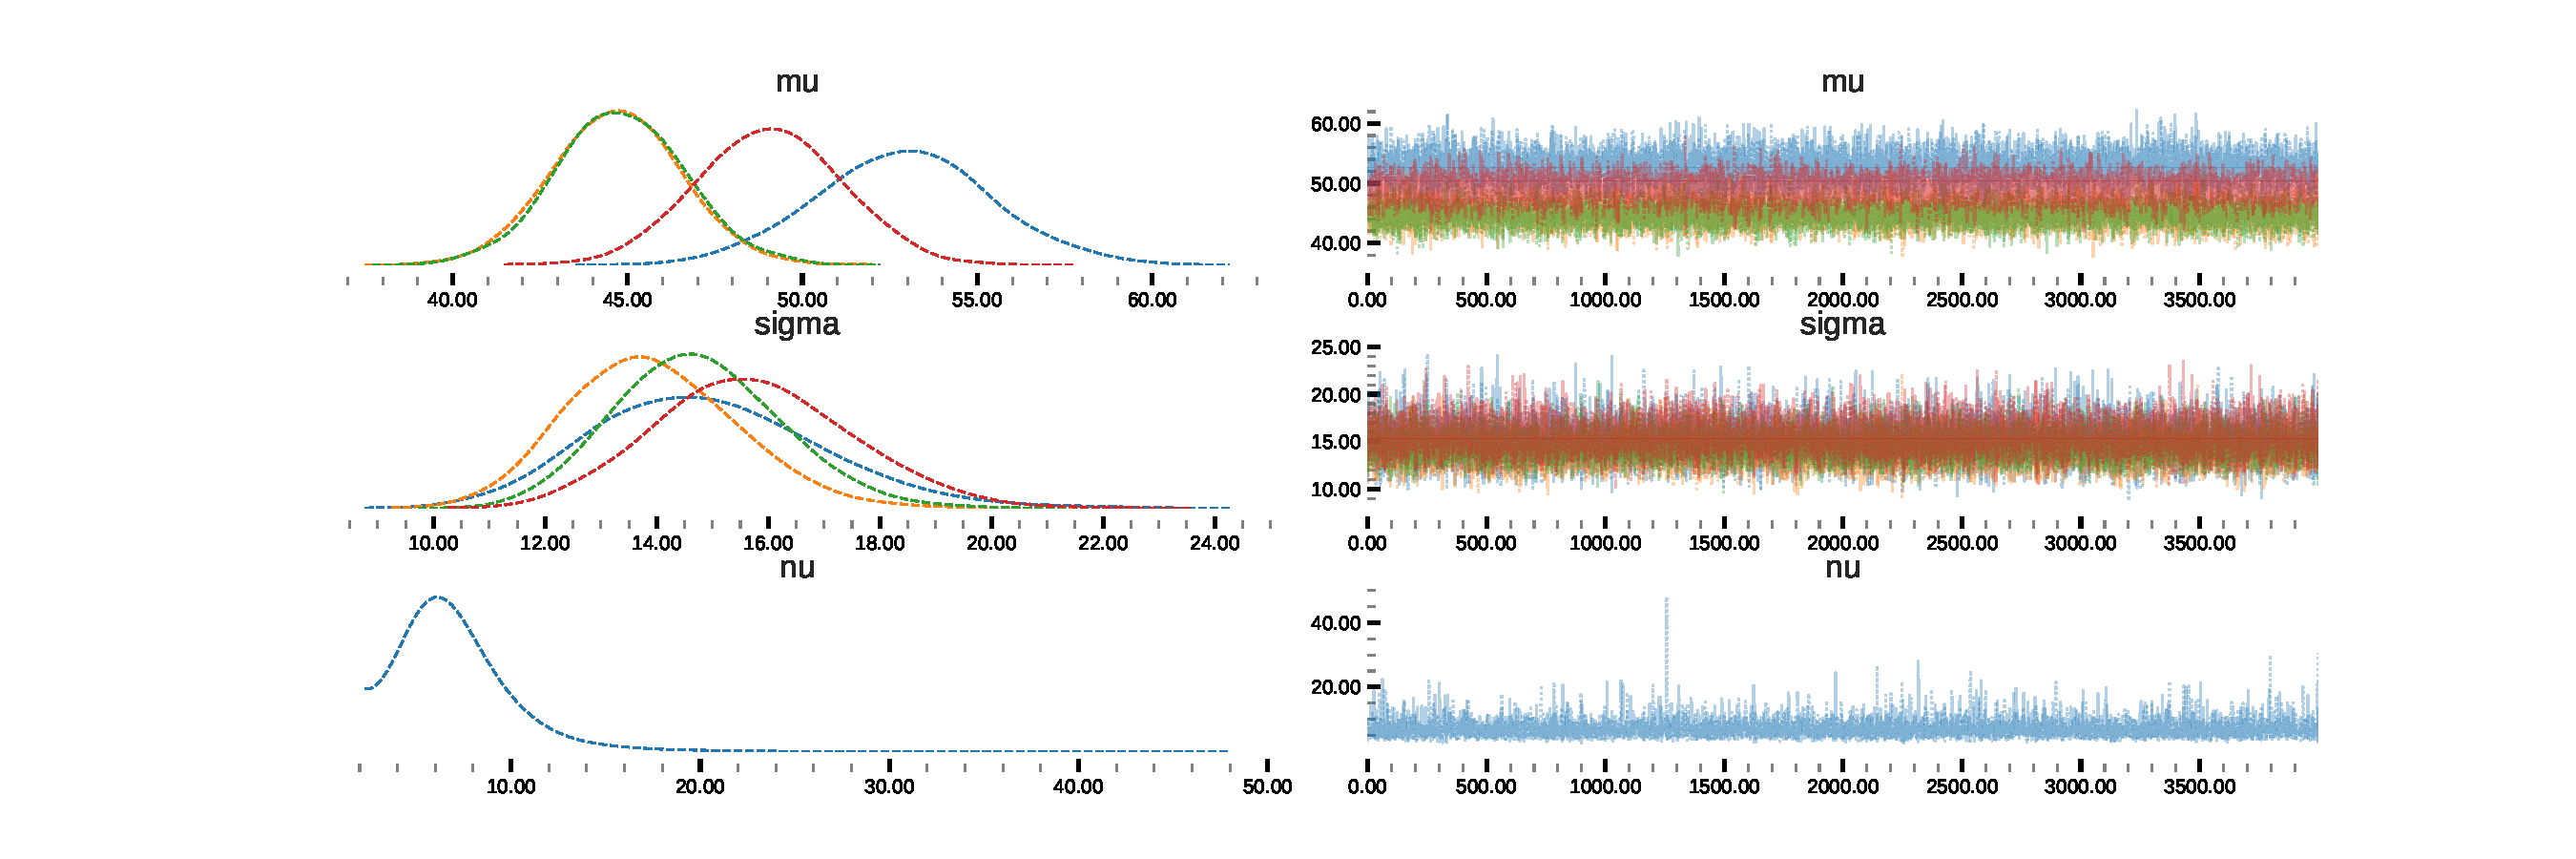
\includegraphics[trim= 2in 0in 2in 0in, clip, width=\textwidth, keepaspectratio=true]{content/image/StudentTIndep_VA_traceplot.pdf}
    \caption{
      Traceplot showing the results of the MCMC estimation. Left column is the posterior distributions for $\mu_{1-4}$, $\sigma_{1-4}$, and $\nu$, and right column shows the corresponding traces. (\lwt{to-do: change to latex expression in figure; more explanation in caption} \tc{add more caption details})
    }
    \Description[Traceplot for experiment 1]{Traceplot for experiment 1}
    \label{fig:traceplot_exp1}
\end{figure}

The Gelman-Rubin statistic $\hat{R}$ for all parameters were 1, 
indicating that the multiple sampling chains converged.
Based on the traceplots in Fig. \ref{fig:traceplot_exp1}, 
the model also shows good convergence. 
The posterior distributions in the left column in Fig. \ref{fig:traceplot_exp1} show that the means of the four Student-t distributions that model the similarity angle, one for each experimental condition, vary. 
In conditions QV108 and QV324 (the overlapping orange and green lines on the left-most side of the four distributions), 
the modes of the mean of the Cosine similarity angle 
(QV108: $44.649 \deg$, QV324: $44.796 \deg$) 
are smaller than those in the other two conditions, 
indicating a better alignment 
between the survey results and donation behavior. 
QV36 (the red line in the middle) has a slightly higher mode of the mean than QV108 and QV324 ($49.029 \deg$), and Likert (the blue line) has the largest mode of the mean ($52.857 \deg$) 
among all four conditions. 
The posterior distributions of the scale parameter $\sigma$
in all four likelihood functions are similar, 
with a mode ranging from $13.904$ and $15.724$. 
(\lwt{to-do: add posterior predictive check in the appendix})

To further confirm how different the means 
of the likelihood functions 
between each pair of the conditions are statistically, 
we constructed the distribution 
of the absolute difference and 
the distribution of the effect size 
(normalized difference) 
between the means as shown in figure \ref{fig:contrast_exp1}.

\begin{figure}[htpb]
  \centering
  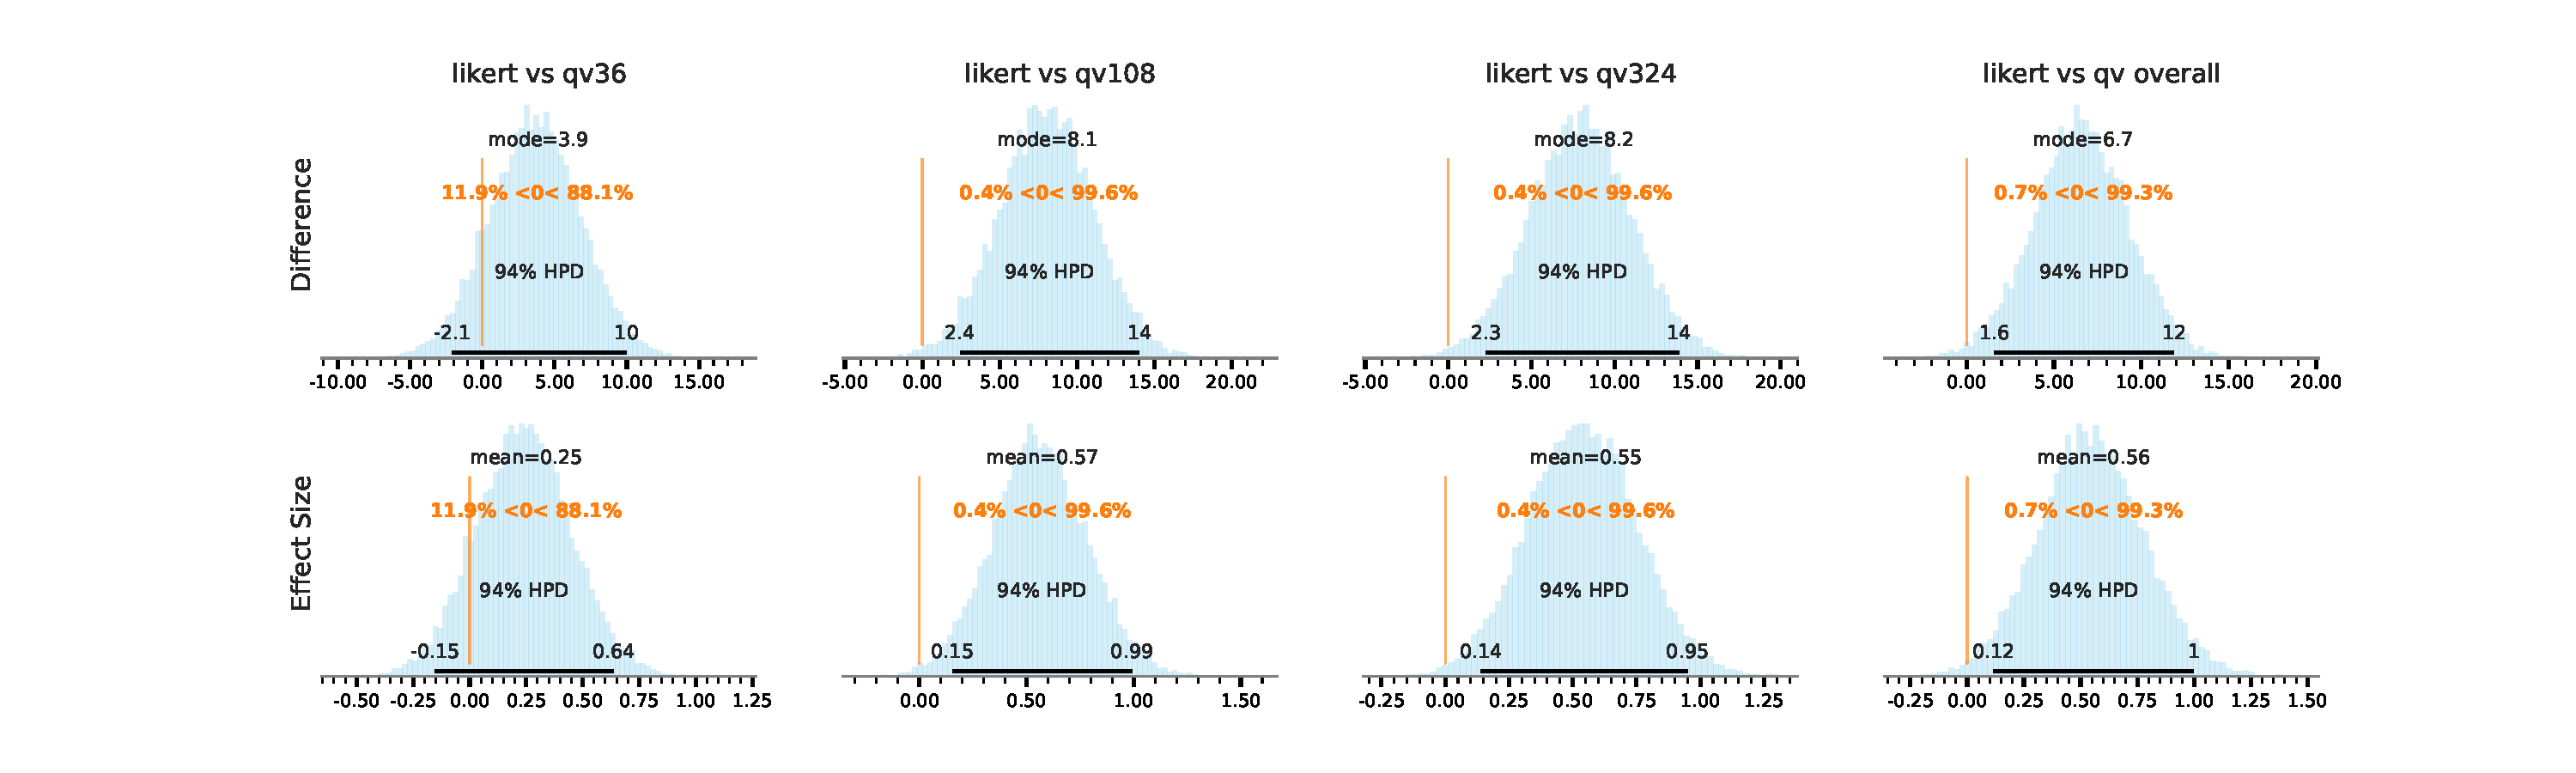
\includegraphics[trim= 2in 0in 2in 0in, clip, width=\textwidth, keepaspectratio=true]{"content/image/Votes_vs_Absolute_Donation_StudentT_differences_and_effects.pdf"}
  \caption{
    The figure shows comparison of the means from the survey-donation alignment likelihood function between the four experimental conditions (Likert donation alignment, QV36 donation alignment, QV108 donation alignment, QV324 donation alignment). The last column shows contrasts between the Likert donation alignment and the pooled QV donation alignment across three QV conditions. The first row focuses on the un-normalized difference while the second row is about the effect size. Since we are highlighting contrasts, each sub-figure shows an orange vertical line located at 0. 
  }
  \Description[Contrasts for experiment 1]{Contrasts for experiment 1}
  \label{fig:contrast_exp1}
\end{figure}

%Is this enough? 
The first column compares the difference between the Likert group
and the donation behavior with the QV group with $36$ votes
with their donation behaviors. We see a mode of $3.9$
with High Posterior Density (HPD) interval of [$-2.1$, $10$].
This implies that the observed differences are not significant.
The model effect size shows a mode of $0.25$, 
with HPD interval of [$-0.15$, $0.64$] 
also indicating the effect size is small.

The second column compares the difference between the Likert group
and the donation behavior with the QV group with 108 votes
with their donation behaviors. We see a mode of $8.1$
with High Posterior Density (HPD) interval of [$2.4$, $14$].
In this case, the HPD lies outside a significant ROPE (Region of Practical Equivalence) of $0 \pm 0.1$
which implies a significant difference that
QV aligns closer to the donation behaviors.
In addition, the effect size shows a mode of $0.57$, 
with HPD interval of [$0.15$, $0.99$] 
indicating a significant, medium effect size.

In the third column, we compare between Likert group
and the donation behavior with the QV group with $324$ votes
with their donation behaviors. We see a mode of $8.2$
with a High Posterior Density (HPD) interval of [$2.3$, $14$].
Again, the HPD lies outside a significant ROPE of $0 \pm 0.1$
which implies a significant difference that
QV aligns closer to the donation behaviors.
The effect size shows a mode of $0.55$, 
with HPD interval of [$0.14$, $0.95$] 
indicating a significant, medium effect size.

The fourth and final column 
compares the difference between the Likert group
and the donation behavior with all three groups of QV
with their donation behaviors. We see a mode of $6.7$
with High Posterior Density (HPD) interval of [$1.6$, $12$].
In this case, the HPD lies outside of ROPE of $0 \pm 0.1$
implies that there is a significant difference where
QV, in general, aligns closer to the donation behaviors.
The effect size shows a mode of $0.56$, 
with HPD interval of [$0.12$, $1.00$] 
indicating a significant, medium effect size.



% Similiar claim that QV allows better alignment to ones true preference
% can be supported by Qualitative Analysis Results.
% We ask participants to provide a freeform text response on the reason why they made the choices they made
% when participants filled out the Likert survey or QV survey,
% Of all surveys ($N=394$) across both groups, most participants filled out the surveys ($N=331$) based on what they think are the most important issues to them. %84 percent
% Besides, a small portion of participants ($N=30$) used their instincts when replying to the survey.
% Some participants either think that every aspect is important ($N=7$) or that resources should be equally distributed ($N=7$). 